\documentclass[11pt]{article}

\usepackage[a4paper,margin=1in]{geometry}
\usepackage{graphicx}
\usepackage{url}
\usepackage{hyperref}
\usepackage{authblk}
\usepackage{color}
\usepackage{amsmath}
\usepackage{fancyvrb}
\usepackage{fontspec}
\setmainfont{TeX Gyre Pagella}
%\setmainfont{TeX Gyre Schola}
\setmonofont{Fira Code}

\title{%
\texttt{Termal}: a fast and interactive terminal-based viewer for multiple sequence alignments
}

\author[1]{Thomas Junier}
\affil[1]{Swiss Institute of Bioinformatics, Vital-\textsc{it} Group, Switzerland\\
\texttt{thomas.junier@sib.swiss}}

\date{} % Actually _suppresses_ the date!

\begin{document}

\maketitle

\begin{abstract} \textbf{Summary:} We present \texttt{termal}, a fast,
  interactive terminal-based viewer for multiple sequence alignments (MSAs),
  designed for use on remote systems such as high-performance computing (HPC)
  clusters. Unlike traditional graphical viewers, \texttt{termal} runs entirely
  within a terminal and offers features such as scrolling, zooming,
  consensus/conservation visualization, and customizable color schemes. It is
  implemented in Rust, ensuring high performance and minimal dependencies.

  \textbf{Availability and implementation:} \texttt{termal} is written in Rust
  and freely available under the MIT license at
  \url{https://github.com/youruser/termal}.

\textbf{Contact:} \texttt{thomas.junier@example.org}
\end{abstract}

\section*{Introduction}

Multiple sequence alignment (MSA) visualization is a common task in
computational biology, yet many tools are GUI-based and unsuitable for use on
headless or remote systems such as HPC clusters. While command-line tools such
as \texttt{showalign} from the EMBOSS suite\cite{emboss} exist, they are limited
in interactivity and display features. \texttt{termal} addresses this gap by
providing a responsive, feature-rich terminal interface for exploring MSAs.
Among terminal-based alignment viewers, Alan\cite{alan} stands out as a
particularly elegant solution, leveraging standard Unix tools such as
\texttt{less} and \texttt{awk} to enable minimalist inspection of multiple
sequence alignments. Indeed, it served as the initial inspiration for the
development of \texttt{termal}. However, Alan is limited by its static output and lack of
interactivity: while scrolling and searching are available through less,
features such as zooming, interactive navigation, consensus/conservation
highlighting, and multiple color schemes are absent.  \texttt{termal} builds on Alan’s
philosophy of terminal-first simplicity, but provides a richer and more
responsive user experience by incorporating a fully interactive terminal UI and
enhanced alignment rendering.

\begin{figure}[htbp]
\centering
	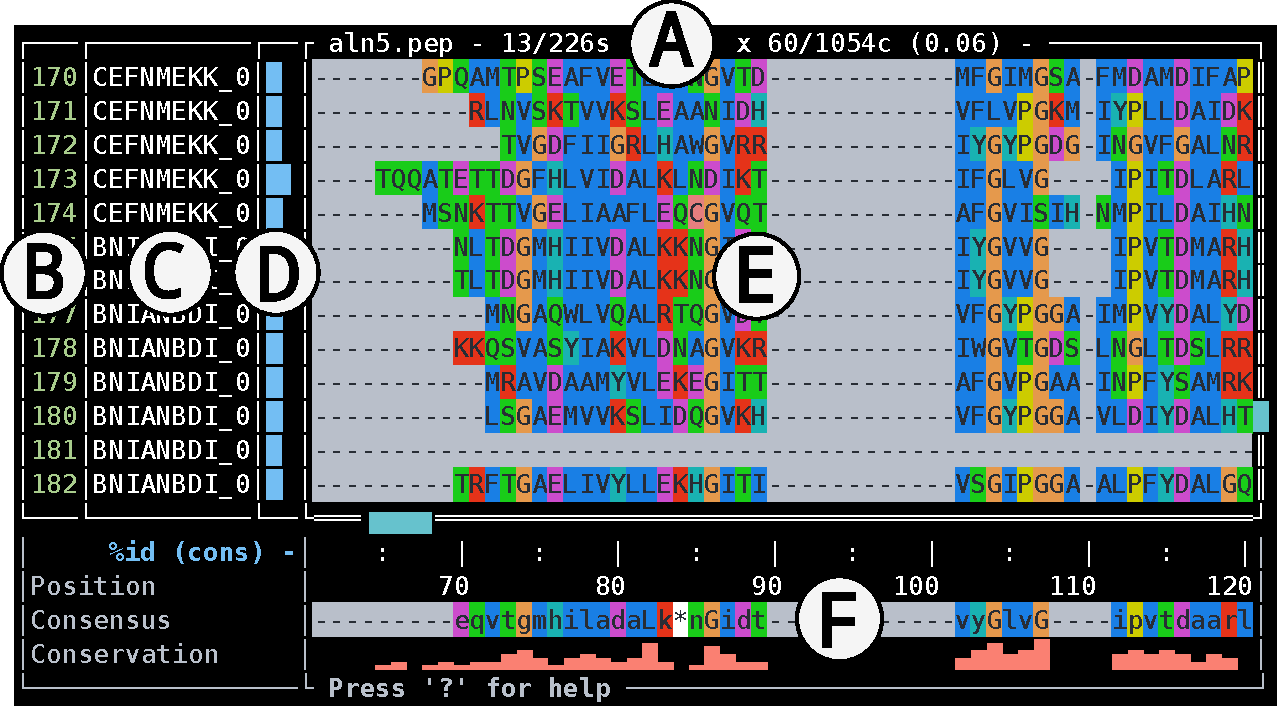
\includegraphics[width=\textwidth]{figure-1.pdf}
\caption{%
	A snapshot of \texttt{termal}'s interface showing a protein alignment. A:
	alignment filename and dimensions, B: sequence numbers pane, C: sequence
	labels pane, D: metric barplot pane (currently displaying sequence similarity
	with the consensus), E: alignment pane, F: bottom pane, displaying sequence
	position, consensus, and conservation barplot. \\
	}
\end{figure}


\section*{Implementation}

\texttt{termal} is implemented in Rust using a modular terminal user interface
(TUI) architecture. It supports common MSA formats such as FASTA and Clustal,
and displays aligned sequences with interactive navigation (keyboard-based
scrolling and zooming), consensus/conservation overlays, and customizable color
schemes. It is distributed as a single static binary for ease of installation
and deployment on remote systems.

\section*{Comparison with Existing Tools}

We compared \texttt{termal} with existing terminal-based viewers including
\texttt{alv} and \texttt{showalign}. Table~\ref{tab:comparison} summarizes their
features.

\begin{table}[h]
\centering
\begin{tabular}{lccc}
\hline
Feature                 & \texttt{termal} & \texttt{alv} & \texttt{showalign} \\
\hline
Terminal-based          & Yes             & Yes          & Yes                \\
Interactive scrolling   & Yes             & Partial      & No                 \\
Zooming                 & Yes             & No           & No                 \\
Color schemes           & Yes             & Basic        & Very limited       \\
Consensus/conservation  & Yes             & Limited      & No                 \\
Format tolerance        & High            & Medium       & Low                \\
Performance (large MSA) & High            & Medium       & Low                \\
\hline
\end{tabular}
\caption{Comparison of \texttt{termal} with other terminal-based MSA viewers.}
\label{tab:comparison}
\end{table}

\section*{Performance and Limits}

\texttt{termal} has been tested on alignments exceeding 15,000 sequences and
1,500 columns (∼22 million alignment cells), with startup and initial rendering
completing in under one second on a machine with 12th-generation
Intel\textregistered{} Core\textsuperscript{TM} i5-1240P CPU and 16 GB of RAM
running Linux 6.14.2. In practice, interactive performance is limited more by
the speed of the terminal emulator than by \texttt{termal} itself.
GPU-accelerated terminals such as Alacritty\cite{alacritty}, Kitty\cite{kitty}
and Ghostty\cite{ghostty} offer smoother scrolling at large screen sizes than do
more traditional emulators.

\section*{Availability}

\texttt{termal} is implemented in Rust and distributed under the MIT license. It
is available as a single precompiled binary for Linux, macOS, and Windows, with
no external dependencies or runtime environment required. Alternatively, users
with Rust installed can install it via \texttt{cargo install termal}.

\section*{Conclusion}

While this work is not intended as a comprehensive review of alignment viewers,
we surveyed several tools with comparable goals — namely, terminal-native
operation and varying degrees of interactivity — including \texttt{showalign},
\texttt{alan}, \texttt{alv}, and \texttt{alen}.  To our knowledge,
\texttt{termal} is the only tool to combine interactive navigation, zooming,
consensus and conservation visualization, and customizable layout options in a
single terminal interface.  Its minimal dependencies and fast startup make
\texttt{termal} suitable for both ad-hoc use and for integration into
semi-automated workflows requiring terminal-based alignment review. Accordingly,
\texttt{termal} fills a niche for fast, interactive MSA exploration directly in
the terminal, making it an ideal tool for remote bioinformatics workflows.

\section*{Funding}

(Optional: include if supported by a grant or institution)

\section*{Acknowledgements}

(Include if you'd like to credit collaborators or contributors)

\bibliographystyle{plain} % or use plainnat, unsrt, etc.
\bibliography{termal}

\end{document}
